\documentclass{article}%文档类型
\usepackage[UTF8]{ctex}%允许中文
\usepackage[a4paper,left=10mm,right=10mm,top=15mm,bottom=15mm]{geometry}%文档布局
\usepackage{titling}%标题包
\usepackage{xcolor}%颜色包
\usepackage{listings}%代码显示包
\usepackage{float}
\usepackage{array}
\usepackage{graphicx}%图像插入包
\usepackage{multirow}
\graphicspath{../}
\renewcommand{\arraystretch}{2} % 增加整体行高
\usepackage{appendix}
\usepackage{hyperref}
\usepackage{amsmath}

%代码显示设置
\lstset{
    language=Python, % 设置语言
    basicstyle={\small\ttfamily}, % 设置字体族
    breaklines=true, % 自动换行
    keywordstyle=\color{blue},  % 关键字样式
    commentstyle=\color{green}, % 注释样式
    stringstyle=\color{red},    % 字符串样式
	emph={self},           % 添加强调词
    emphstyle=\color{blue}\bfseries, % 强调词样式
    columns=flexible,
    numbers=left, % 显示行号在左边
    numbersep=2em, % 设置行号的具体位置
    numberstyle=\footnotesize, % 缩小行号
    frame=single, % 边框
    framesep=1em, % 设置代码与边框的距离
	xleftmargin=2em, % 左边距
    xrightmargin=2em, % 右边距
    escapeinside=``,
}

\title{视听信息系统导论第三次编程作业报告}

\begin{document}
%标题页
\begin{titlepage}
    \thispagestyle{empty}
    \vspace*{4cm} % 顶部填充
    \begin{center}
    {\LARGE \textbf{\thetitle}}\\
    \vspace{6cm}
    \end{center}
    \vspace*{\fill} % 底部填充
\end{titlepage}

\zihao{-4}
\setlength{\baselineskip}{22pt}
\tableofcontents
\clearpage

\section{实验任务}

\subsection{数据准备}
\subsubsection{TASK 1}
补全 dataset.py 中的 prepare\_data 函数,并详细说明整个函数是如何构建词表的。

函数代码如下:
\begin{lstlisting}
def prepare_data(data_path):
    with open(data_path) as f:
        data = f.read()

    ################################################################################
    # TODO: insert '#' at the end of each paragraph, delete all special chars;     #
    #  you can leverage data.replace() and data.split() to accomplish that.        #
    #  two or three lines of code should be sufficient.                            #
    ################################################################################
    # *****START OF YOUR CODE (DO NOT DELETE/MODIFY THIS LINE)*****

    data = data.replace('\n\n', '#')
    data = '` `'.join(data.split())
    
    # *****END OF YOUR CODE (DO NOT DELETE/MODIFY THIS LINE)*****
    ################################################################################
    #                              END OF YOUR CODE                                #
    ################################################################################
\end{lstlisting}

其中词表的构建流程是:

首先对数据进行预处理。

再提取唯一字符集合:\verb|unique_chars = set(data)|。

将每个字符映射为一个唯一索引:\verb|voc2ind[char] = idx|。

再创建反向映射:\verb|ind2voc = {val: key for key, val in voc2ind.items()}|。

将data按80\%和20\%分割成训练集和测试集,使用\verb|voc2ind[char]|将训练集和测试集中的每个字符转换为对应的整数索引。

将训练集和测试集的整数表示、字符到索引的正向映射、字符到索引的反向映射保存下来。

\subsubsection{TASK 2}
请完成 dataset.py 中的 HarryPotterDataset 类。(完成代码即可,不用在报告中写文字说明)

代码如下:
\begin{lstlisting}
class HarryPotterDataset(torch.utils.data.Dataset):
    def __init__(self, data_file, sequence_length, batch_size):
        super(HarryPotterDataset, self).__init__() 

        self.sequence_length = sequence_length
        self.batch_size = batch_size
        self.vocab = Vocabulary(data_file)

        with open(data_file, 'rb') as data_pkl:
            dataset = pickle.load(data_pkl)
        
        self.tokens = dataset['tokens']
        self.voc2ind = dataset['voc2ind']
        self.ind2voc = dataset['ind2voc']

        self.data = None
        self.sequences_in_batch = None
        ################################################################################
        # TODO: split self.tokens to len(self.tokens)//batch_size chunks, store the    #
        #  reshaped data (and convert it to torch.LongTensor) in self.data;            #
        #  Then compute how many sequences are there in each chunk, store that in      #
        #  self.sequences_in_batch                                                     #
        ################################################################################
        # *****START OF YOUR CODE (DO NOT DELETE/MODIFY THIS LINE)*****

        self.data = torch.LongTensor(self.tokens[:len(self.tokens) // self.batch_size * self.batch_size])
        self.data = self.data.view(self.batch_size, -1)
        self.sequences_in_batch = self.data.size(1) // self.sequence_length

        # *****END OF YOUR CODE (DO NOT DELETE/MODIFY THIS LINE)*****
        ################################################################################
        #                              END OF YOUR CODE                                #
        ################################################################################

    def __len__(self):
        ################################################################################
        # TODO: return the total number of sequences in dataset                        #
        ################################################################################
        # *****START OF YOUR CODE (DO NOT DELETE/MODIFY THIS LINE)*****
        
        return self.sequences_in_batch * self.batch_size

        # *****END OF YOUR CODE (DO NOT DELETE/MODIFY THIS LINE)*****
        ################################################################################
        #                              END OF YOUR CODE                                #
        ################################################################################
        
    def __getitem__(self, idx):
        data = None
        ################################################################################
        # TODO: Based on idx, determine the chunk idx and the sequence idx of the chunk#
        #  fetch that sequence data from self.data and store that in data variable;    #
        #  Note the data length should be sequence_length + 1                          #
        ################################################################################
        # *****START OF YOUR CODE (DO NOT DELETE/MODIFY THIS LINE)*****

        chunk_idx = idx // self.sequences_in_batch
        seq_idx = idx % self.sequences_in_batch
        start = seq_idx * self.sequence_length
        end = start + self.sequence_length + 1
        data = self.data[chunk_idx, start:end]

        # *****END OF YOUR CODE (DO NOT DELETE/MODIFY THIS LINE)*****
        ################################################################################
        #                              END OF YOUR CODE                                #
        ################################################################################

        # returns input data and label data (next token of input) with their length sequence_length
        return data[:-1], data[1:]

    def vocab_size(self):
        return len(self.vocab)
\end{lstlisting}

\subsection{构建模型}
\subsubsection{TASK 3}
请完成 model.py 中的 HarryPotterTransformer 类。(完成代码即可,不用在报告中写文字说明)
请基于构建的网络完成训练,绘制训练、测试的损失曲线和测试的准确率曲线。(请绘制在报告中)

代码如下:
\begin{lstlisting}
class HarryPotterTransformer(nn.Module):
    def __init__(self, vocab_size, feature_size, num_heads):
        super(HarryPotterTransformer, self).__init__()
        self.vocab_size = vocab_size
        self.feature_size = feature_size
        self.num_heads = num_heads
        self.best_accuracy = -1

        self.embedding = None
        self.transformer_encoder = None
        self.decoder = None
        self.pos_encoding = None # you can omit this for Task 4

        ################################################################################
        # TODO: define the network                                                     #
        ################################################################################
        # *****START OF YOUR CODE (DO NOT DELETE/MODIFY THIS LINE)*****

        self.embedding = nn.Embedding(vocab_size, feature_size)
        encoder_layer = nn.TransformerEncoderLayer(
            d_model=feature_size,
            nhead=num_heads,
            dim_feedforward=4 * feature_size,
            dropout=0.1
        )
        self.transformer_encoder = nn.TransformerEncoder(encoder_layer, num_layers=2)
        self.decoder = nn.Linear(feature_size, vocab_size)
        self.pos_encoding = PositionalEncoding(feature_size)

        # *****END OF YOUR CODE (DO NOT DELETE/MODIFY THIS LINE)*****
        ################################################################################
        #                              END OF YOUR CODE                                #
        ################################################################################

    def forward(self, x):        
        attn_mask = None # you can omit this for Task 4 and Task 5
        ################################################################################
        # TODO: finish the forward pass                                                #
        ################################################################################
        # *****START OF YOUR CODE (DO NOT DELETE/MODIFY THIS LINE)*****

        x = self.embedding(x) # [batch_size, seq_len, feature_size]
        x = x.permute(1, 0, 2) # [seq_len, batch_size, feature_size]
        x = self.transformer_encoder(x, mask=attn_mask) # [seq_len, batch_size, feature_size]
        x = x.permute(1, 0, 2) # [batch_size, seq_len, feature_size]
        x = self.decoder(x) # [batch_size, seq_len, vocab_size]

        # *****END OF YOUR CODE (DO NOT DELETE/MODIFY THIS LINE)*****
        ################################################################################
        #                              END OF YOUR CODE                                #
        ################################################################################

        return x
\end{lstlisting}

得到的模型训练、测试的损失曲线和测试的准确率曲线如下:
\begin{figure}[H]
    \centering
    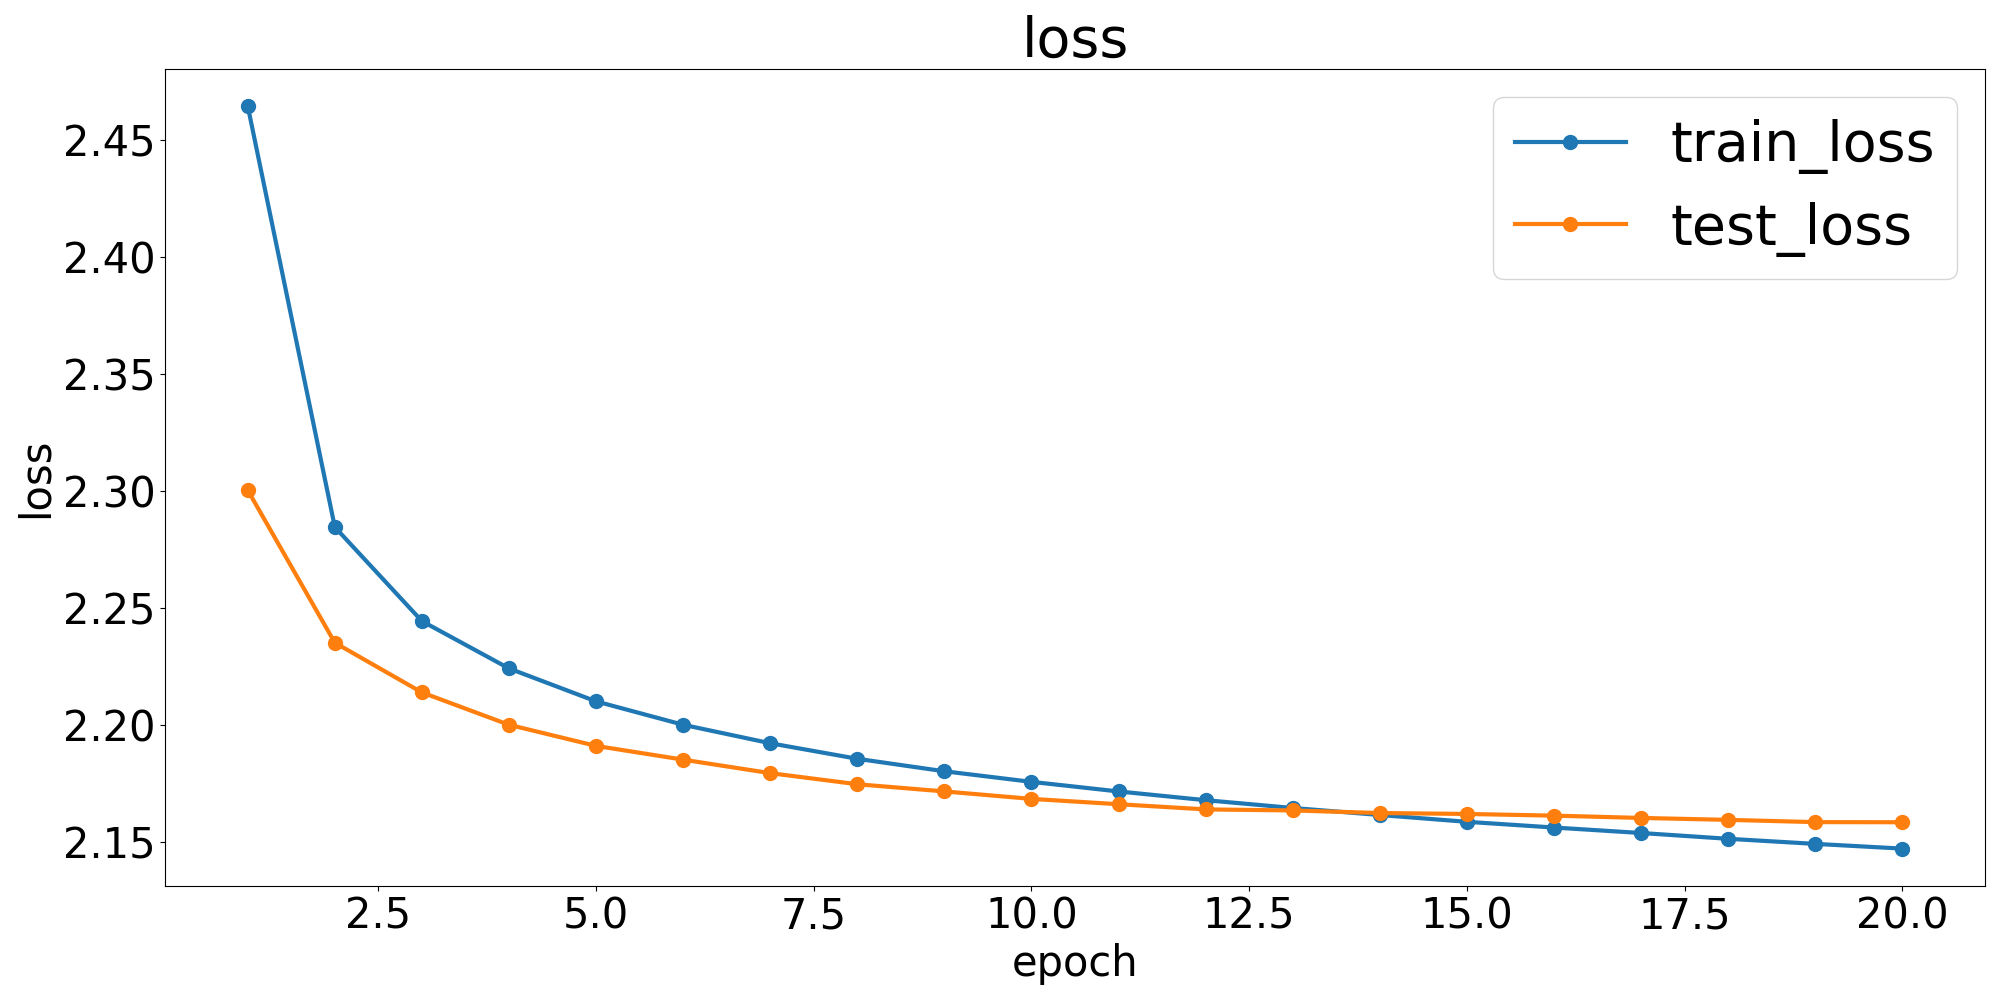
\includegraphics[width=0.9\linewidth]{../exp_task3/figs/loss.png}
    \caption{Loss曲线}
\end{figure}
\begin{figure}[H]
    \centering
    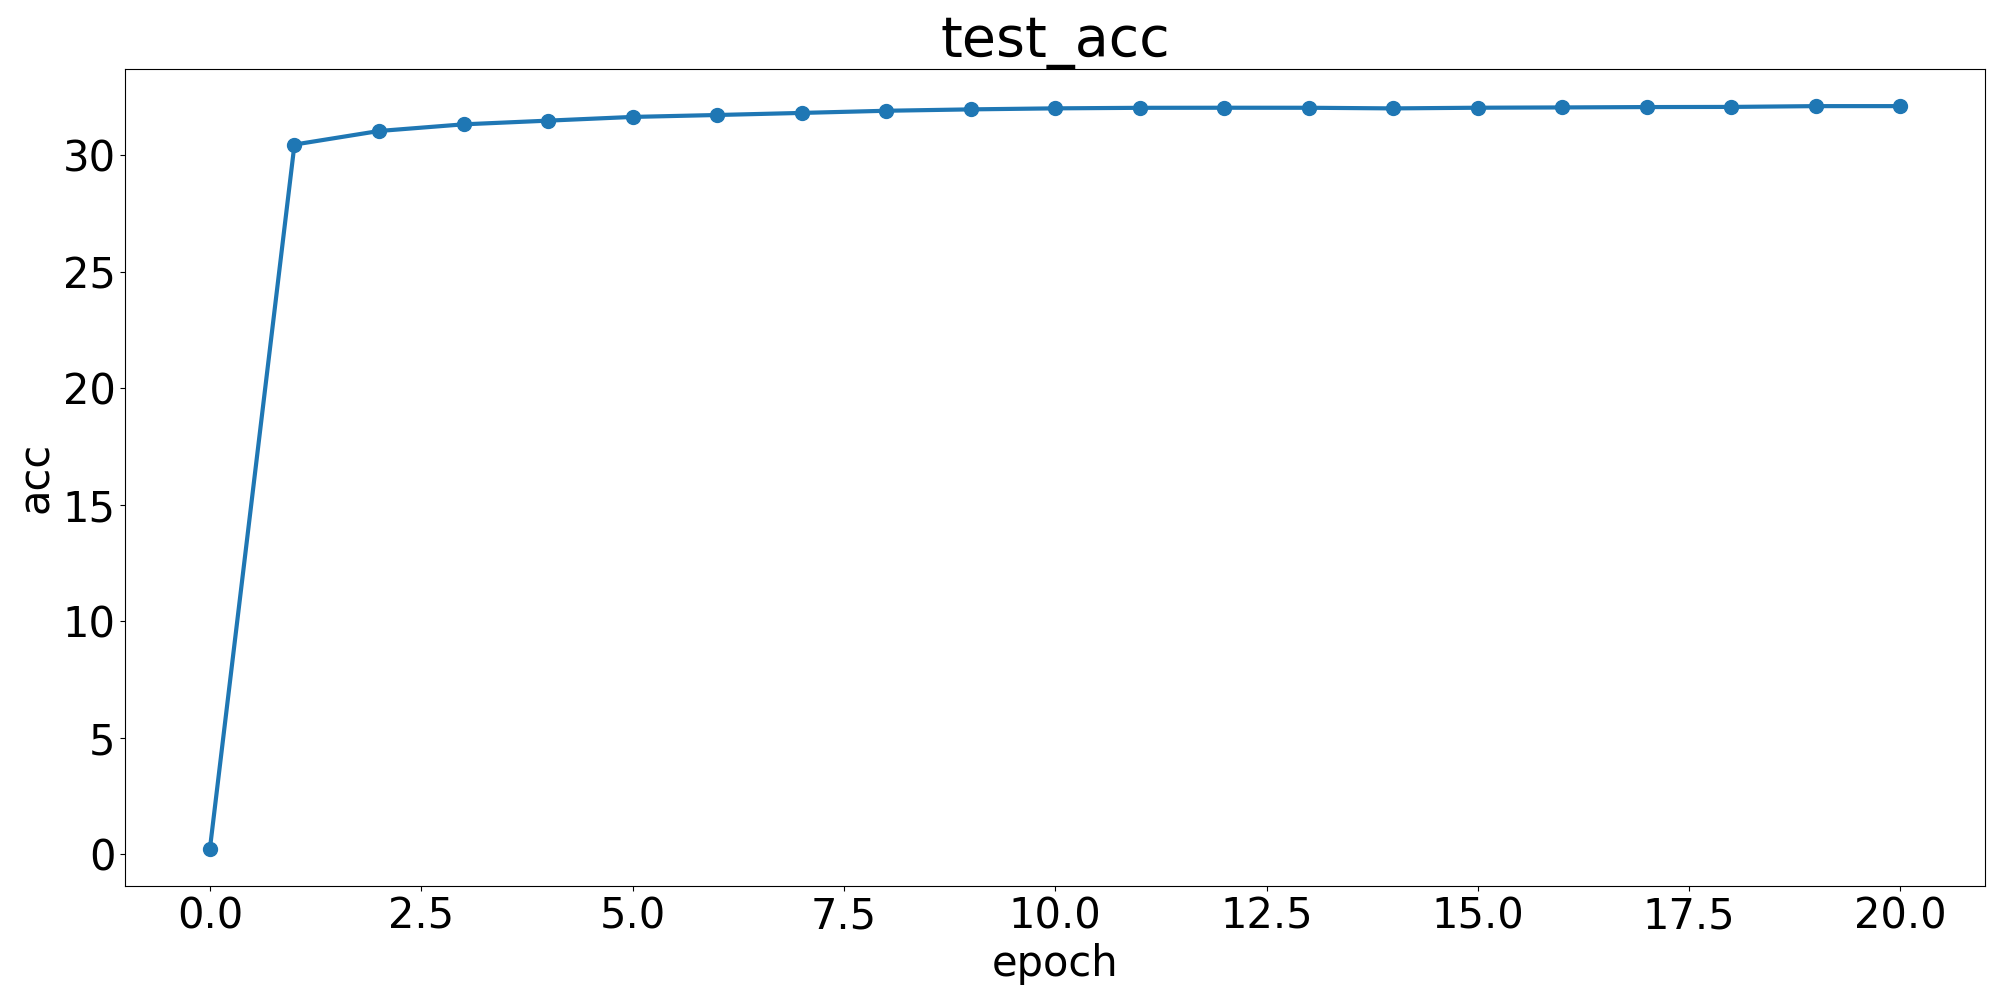
\includegraphics[width=0.9\linewidth]{../exp_task3/figs/test_acc.png}
    \caption{Acc曲线}
\end{figure}

\subsubsection{TASK 4}
请完成 model.py 中的 PositionalEncoding 类并将其加入到 HarryPotterTransformer 类中。(完
成代码即可,不用在报告中写文字说明)
请基于构建的网络完成训练,绘制训练、测试的损失曲线和测试的准确率曲线,并且分析 positional
encoding 的作用。(请绘制在报告中)

代码如下:
\begin{lstlisting}
class PositionalEncoding(nn.Module):
    def __init__(self, d_model, max_len = 5000):
        super().__init__()
        pe = None
        ################################################################################
        # TODO: compute the positional encoding                                        #
        ################################################################################
        # *****START OF YOUR CODE (DO NOT DELETE/MODIFY THIS LINE)*****

        pe = torch.zeros(max_len, d_model)
        position = torch.arange(0, max_len).unsqueeze(1)
        div_term = torch.exp(torch.arange(0, d_model, 2) * (-math.log(10000.0) / d_model))
        pe[:, 0::2] = torch.sin(position * div_term)
        pe[:, 1::2] = torch.cos(position * div_term)

        # *****END OF YOUR CODE (DO NOT DELETE/MODIFY THIS LINE)*****
        ################################################################################
        #                              END OF YOUR CODE                                #
        ################################################################################
        self.register_buffer('pe', pe)

    def forward(self, x):
        """
        Arguments:
            x: Tensor, shape ``[batch_size, seq_len, embedding_dim]``
        """
        x = x + self.pe.unsqueeze(0)[:, :x.size(1)]
        return x

class HarryPotterTransformer(nn.Module):
    def forward(self, x):        
        attn_mask = None # you can omit this for Task 4 and Task 5
        ################################################################################
        # TODO: finish the forward pass                                                #
        ################################################################################
        # *****START OF YOUR CODE (DO NOT DELETE/MODIFY THIS LINE)*****

        x = self.embedding(x) # [batch_size, seq_len, feature_size]
        x = self.pos_encoding(x) # [batch_size, seq_len, feature_size], Added in Task 4
        x = x.permute(1, 0, 2) # [seq_len, batch_size, feature_size]
        x = self.transformer_encoder(x, mask=attn_mask) # [seq_len, batch_size, feature_size]
        x = x.permute(1, 0, 2) # [batch_size, seq_len, feature_size]
        x = self.decoder(x) # [batch_size, seq_len, vocab_size]

        # *****END OF YOUR CODE (DO NOT DELETE/MODIFY THIS LINE)*****
        ################################################################################
        #                              END OF YOUR CODE                                #
        ################################################################################

        return x
\end{lstlisting}

得到的模型训练、测试的损失曲线和测试的准确率曲线如下:
\begin{figure}[H]
    \centering
    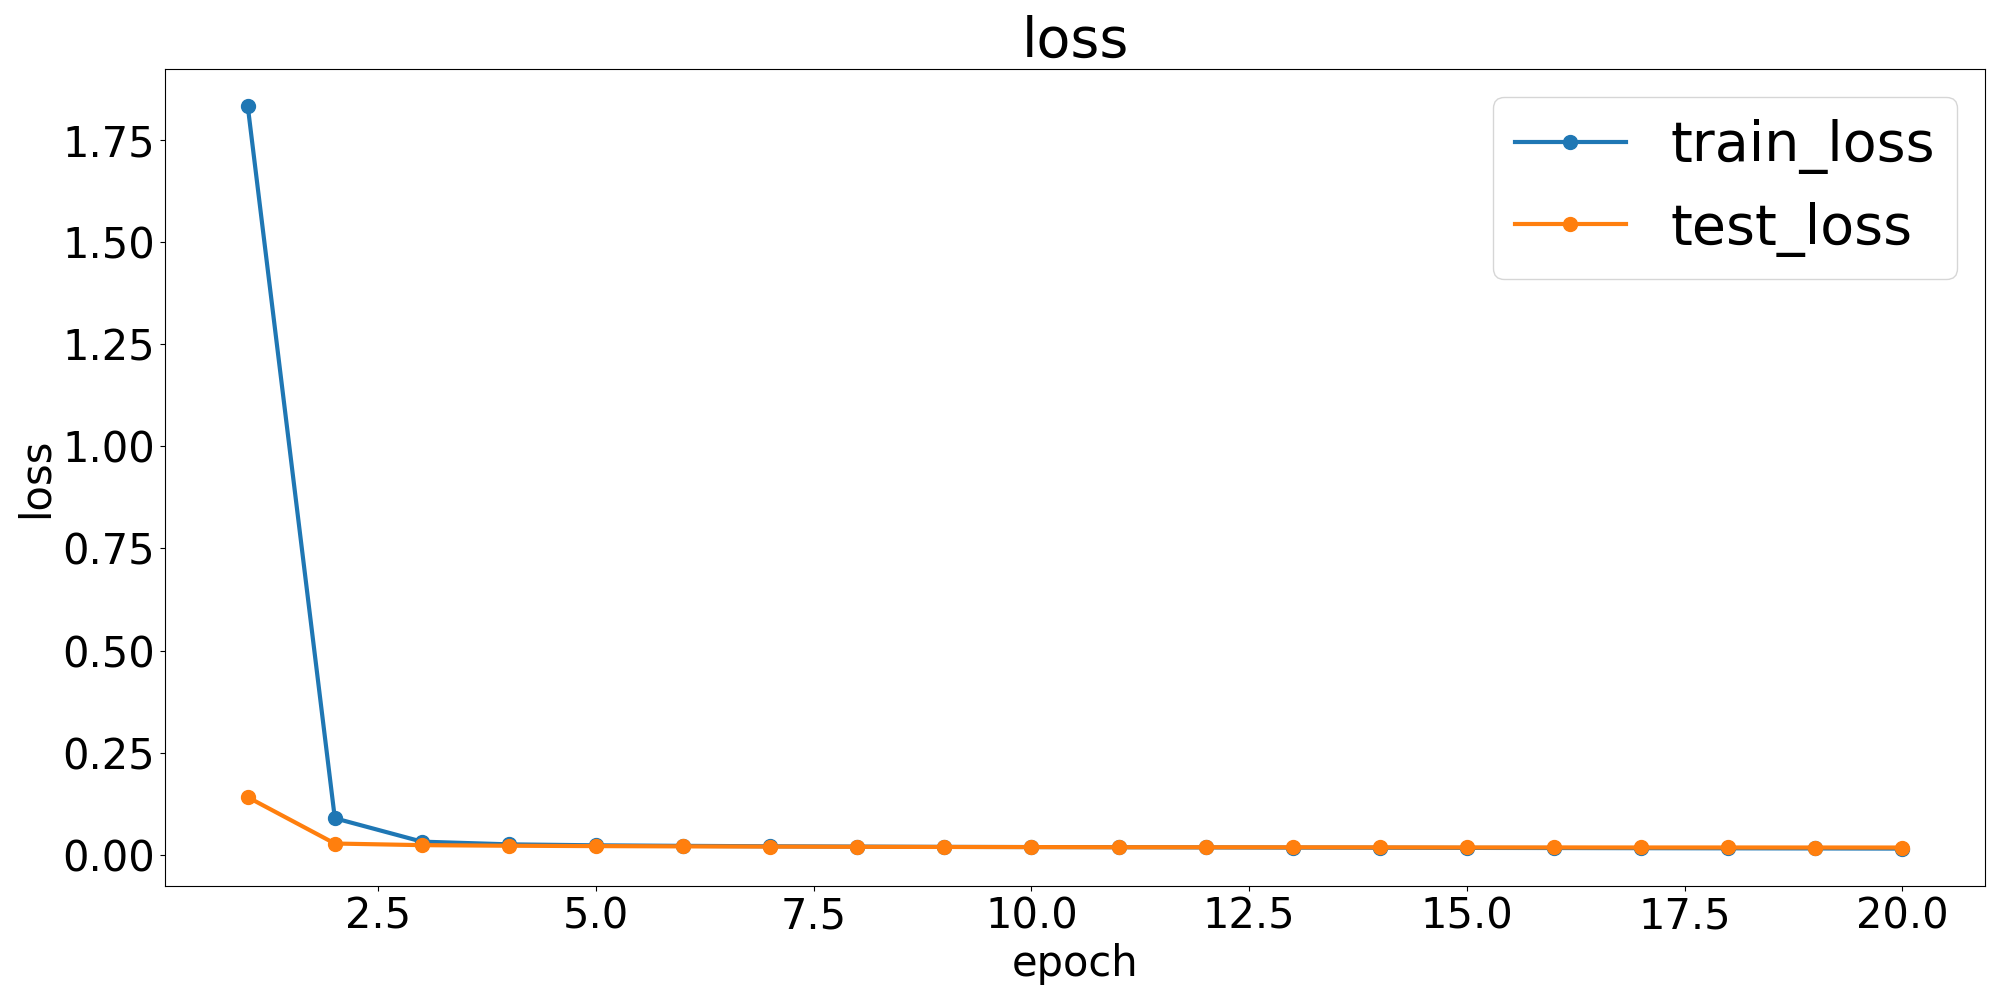
\includegraphics[width=0.9\linewidth]{../exp_task4/figs/loss.png}
    \caption{Loss曲线}
\end{figure}
\begin{figure}[H]
    \centering
    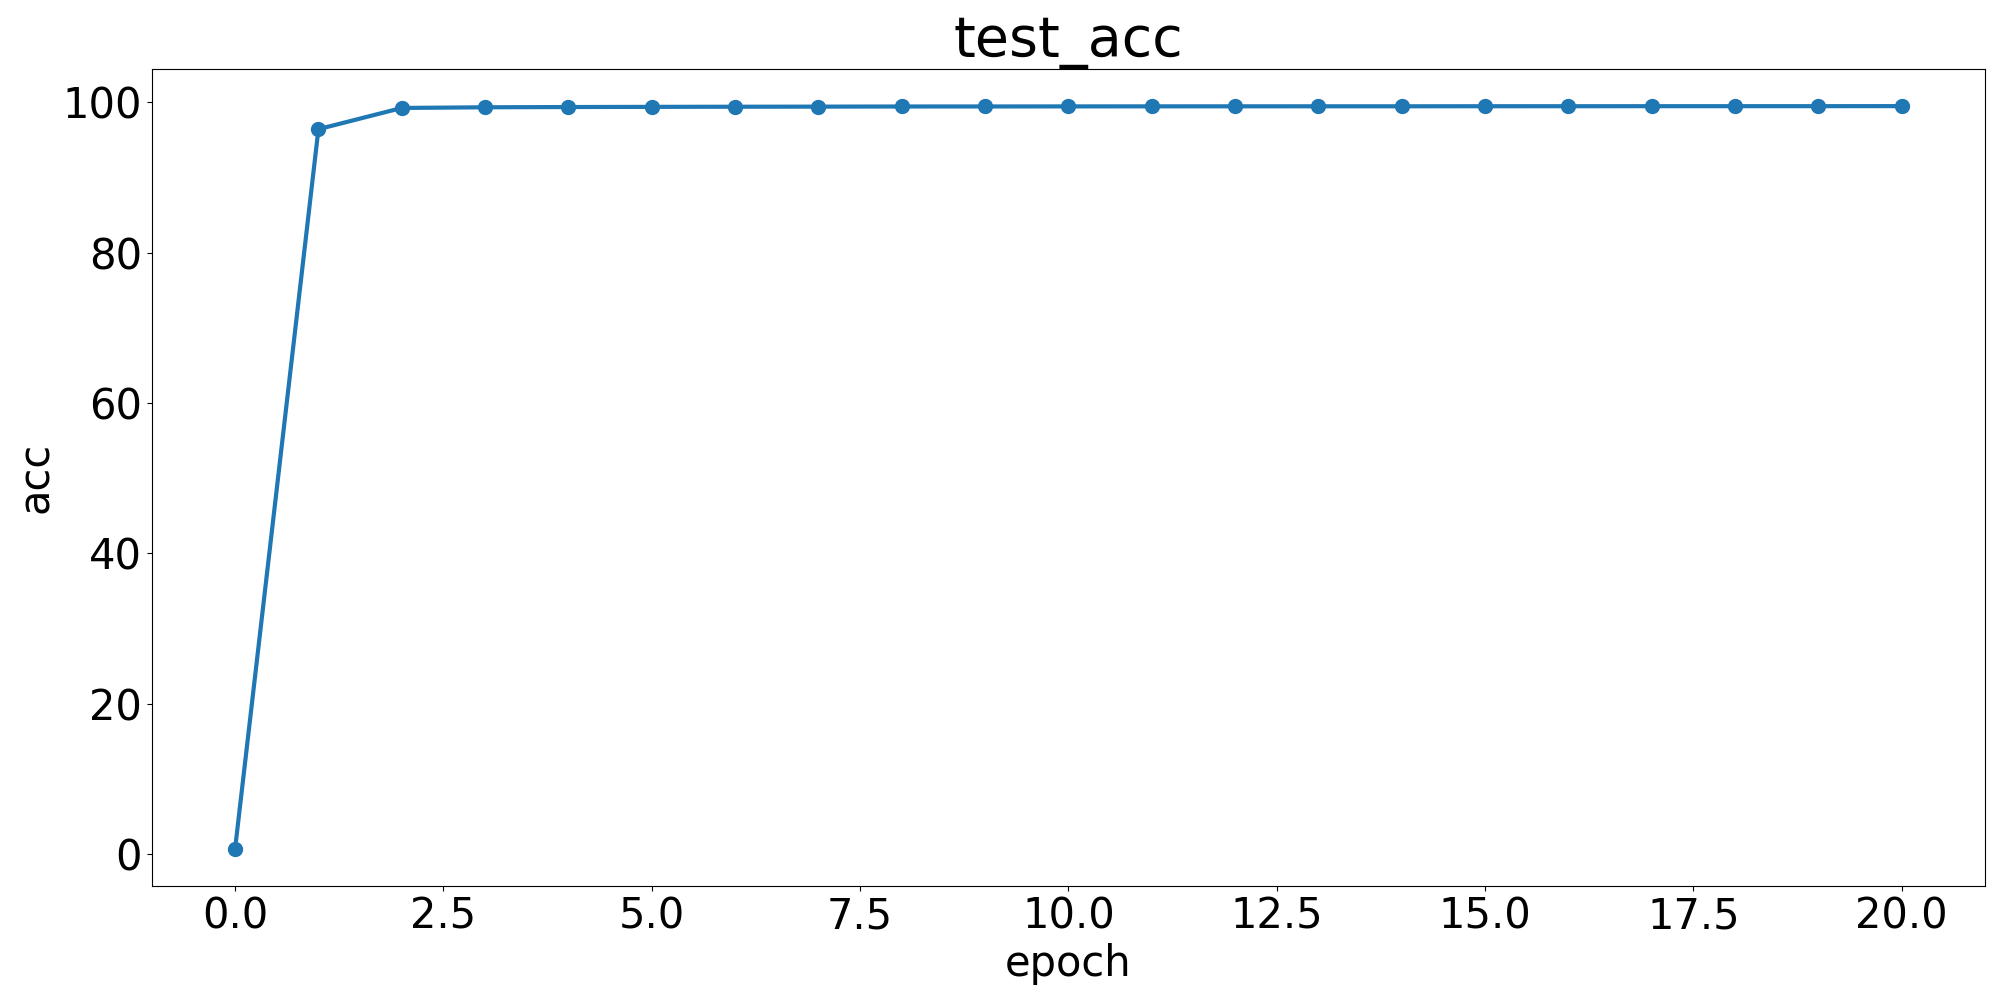
\includegraphics[width=0.9\linewidth]{../exp_task4/figs/test_acc.png}
    \caption{Acc曲线}
\end{figure}

可以看到再使用了PositionalEncoding后,Loss曲线下降显著加快,
PositionalEncoding为输入序列中的每个位置引入位置信息,从而弥补自注意力机制对序列顺序缺失的不足。
但是曲线还是很奇怪,Loss下降速度过快,原因是因为没有使用attention mask防止训练和测试时使用未来的文本数据。

\subsubsection{TASK 5}
请实现 attention mask 并将其加入到 HarryPotterTransformer 类的 forward 函数中。(完成代
码即可,不用在报告中写文字说明)
请基于构建的网络完成训练,绘制训练、测试的损失曲线和测试的准确率曲线,并且分析 attention
mask 的作用。(请绘制在报告中)

代码如下:
\begin{lstlisting}
class HarryPotterTransformer(nn.Module):
    def forward(self, x):        
        attn_mask = None # you can omit this for Task 4 and Task 5
        ################################################################################
        # TODO: finish the forward pass                                                #
        ################################################################################
        # *****START OF YOUR CODE (DO NOT DELETE/MODIFY THIS LINE)*****

        x = self.embedding(x) # [batch_size, seq_len, feature_size]
        x = self.pos_encoding(x) # [batch_size, seq_len, feature_size], Added in Task 4
        x = x.permute(1, 0, 2) # [seq_len, batch_size, feature_size]
        attn_mask = torch.triu(torch.ones(x.size(0), x.size(0)), diagonal=1).to(x.device) # Added in Task 5
        attn_mask = attn_mask.masked_fill(attn_mask == 1, float('-inf')) # Added in Task 5
        x = self.transformer_encoder(x, mask=attn_mask) # [seq_len, batch_size, feature_size]
        x = x.permute(1, 0, 2) # [batch_size, seq_len, feature_size]
        x = self.decoder(x) # [batch_size, seq_len, vocab_size]

        # *****END OF YOUR CODE (DO NOT DELETE/MODIFY THIS LINE)*****
        ################################################################################
        #                              END OF YOUR CODE                                #
        ################################################################################

        return x
\end{lstlisting}

得到的模型训练、测试的损失曲线和测试的准确率曲线如下:
\begin{figure}[H]
    \centering
    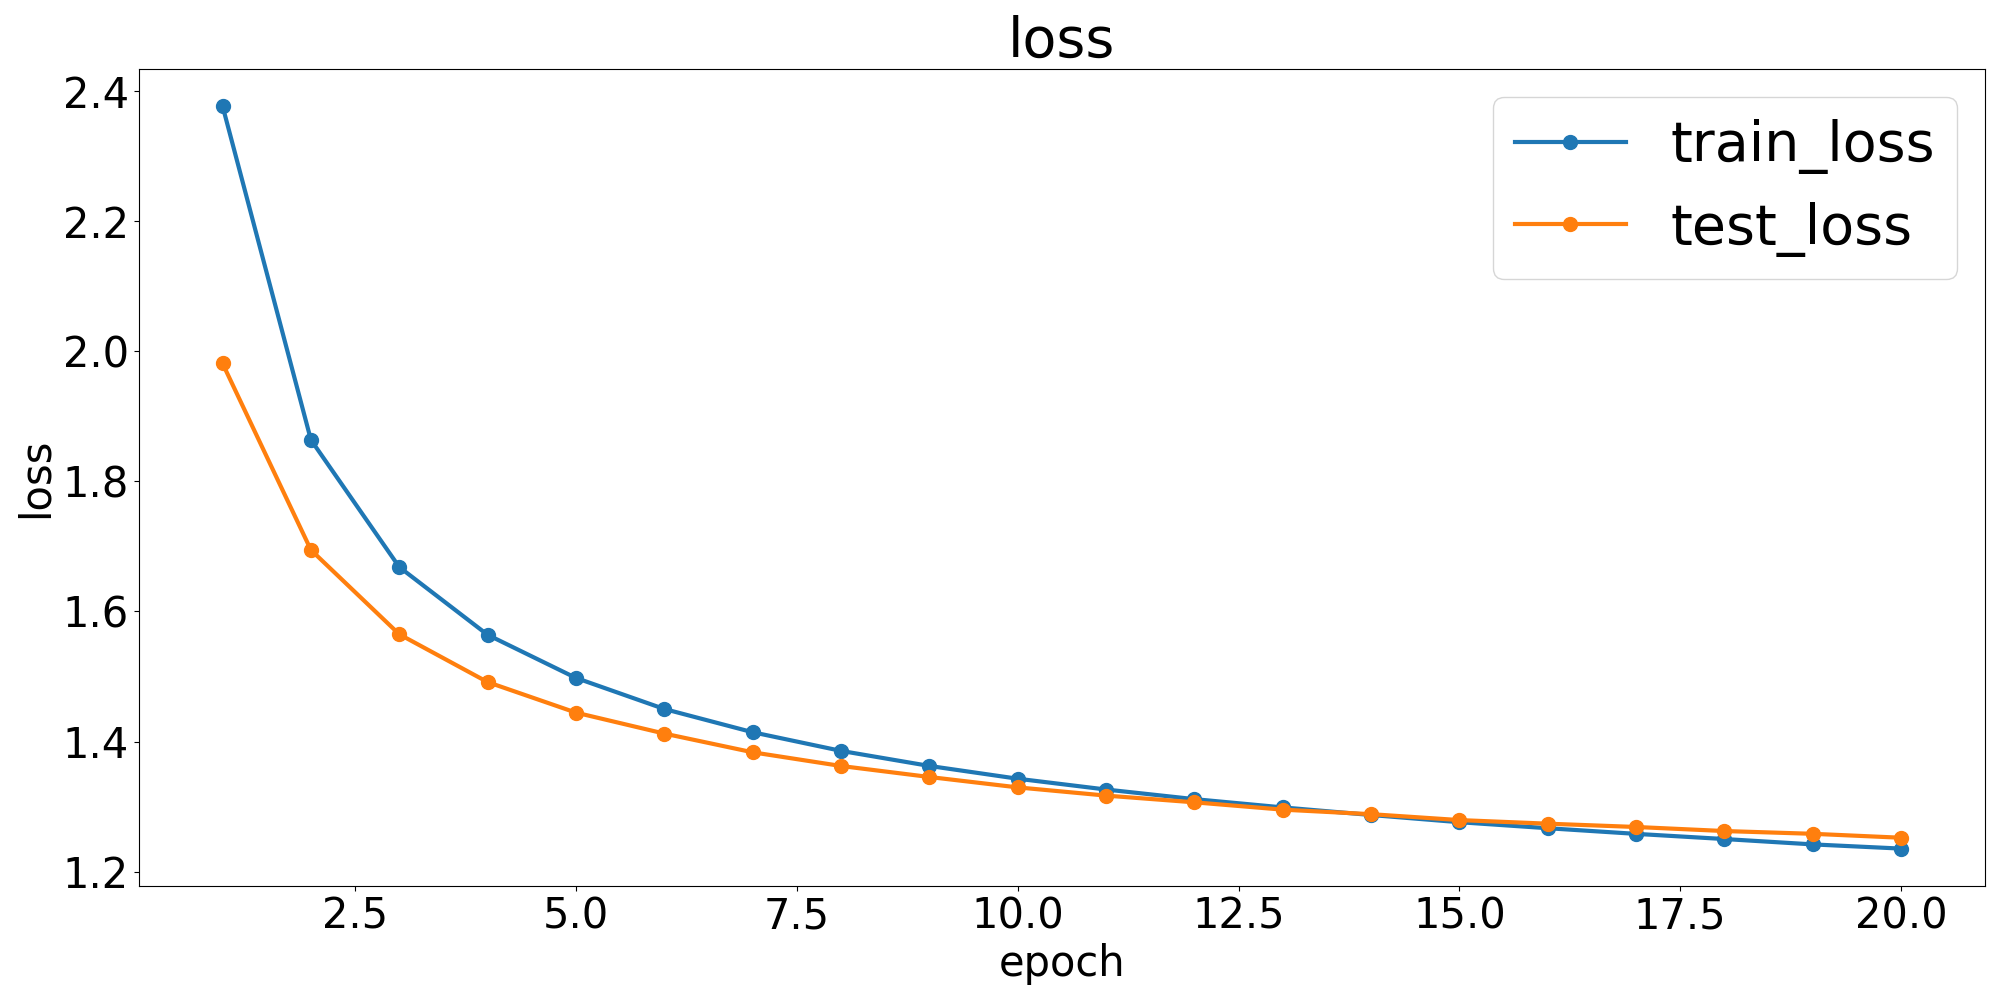
\includegraphics[width=0.9\linewidth]{../exp_task5/figs/loss.png}
    \caption{Loss曲线}
\end{figure}
\begin{figure}[H]
    \centering
    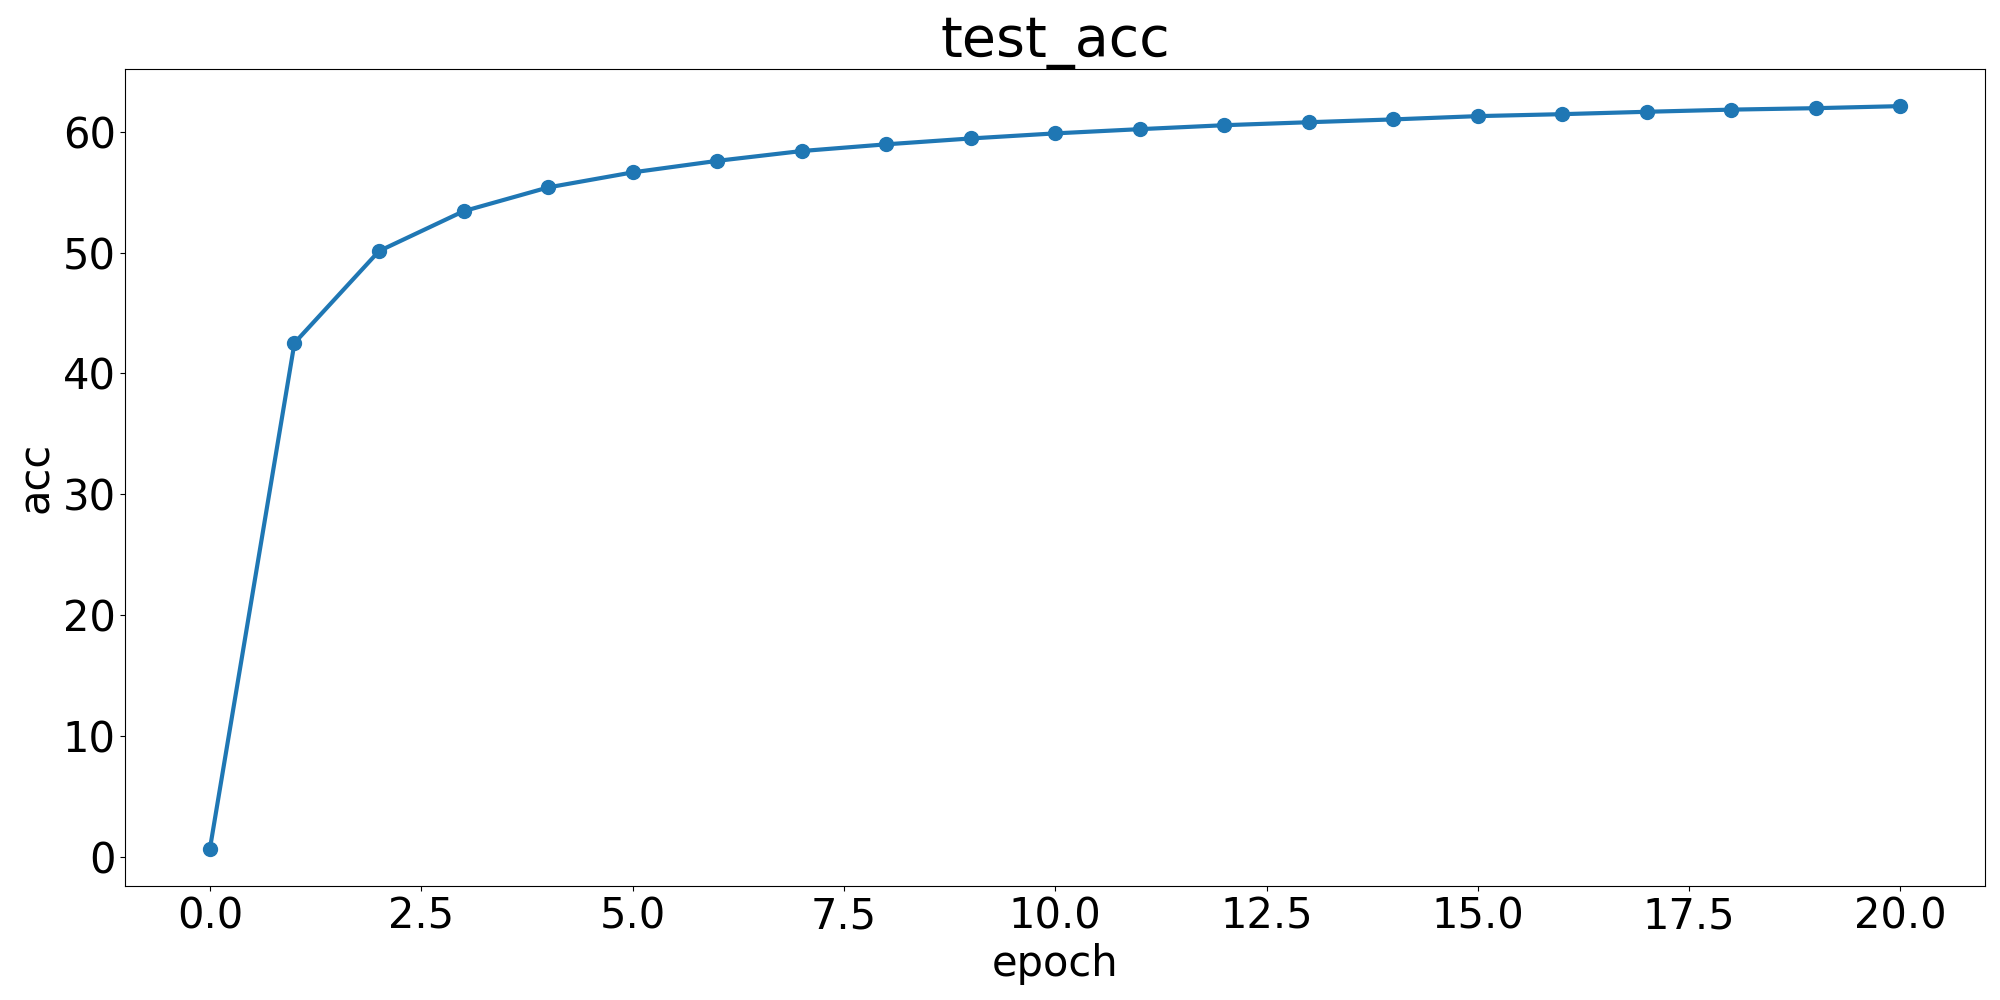
\includegraphics[width=0.9\linewidth]{../exp_task5/figs/test_acc.png}
    \caption{Acc曲线}
\end{figure}

使用attention mask之后,Loss曲线变得更加正常,没有急速下降。attention mask的作用是防止模型访问未来时间步的信息。
如果模型访问了未来时间步的信息,将导致目标值泄露,破坏训练。

\subsection{文本生成}
\subsubsection{TASK 6}
在默认参数(temperature=1, strategy='sampling')下,调整模型生成使用的seed\_words,将
你最喜欢的生成结果附在报告中。

seed\_words调整如下:
\begin{lstlisting}
    # generate
    # Try different seed_words. Find interesting ones.
    seed_words = "Harry Potter came to Tsinghua University and attended a course named Introduction to Auditory Visual Information System. "
    # Experiment with different temperatures to observe their impact on diversity and stability.
\end{lstlisting}
得到的生成如下:
\begin{figure}[H]
    \centering
    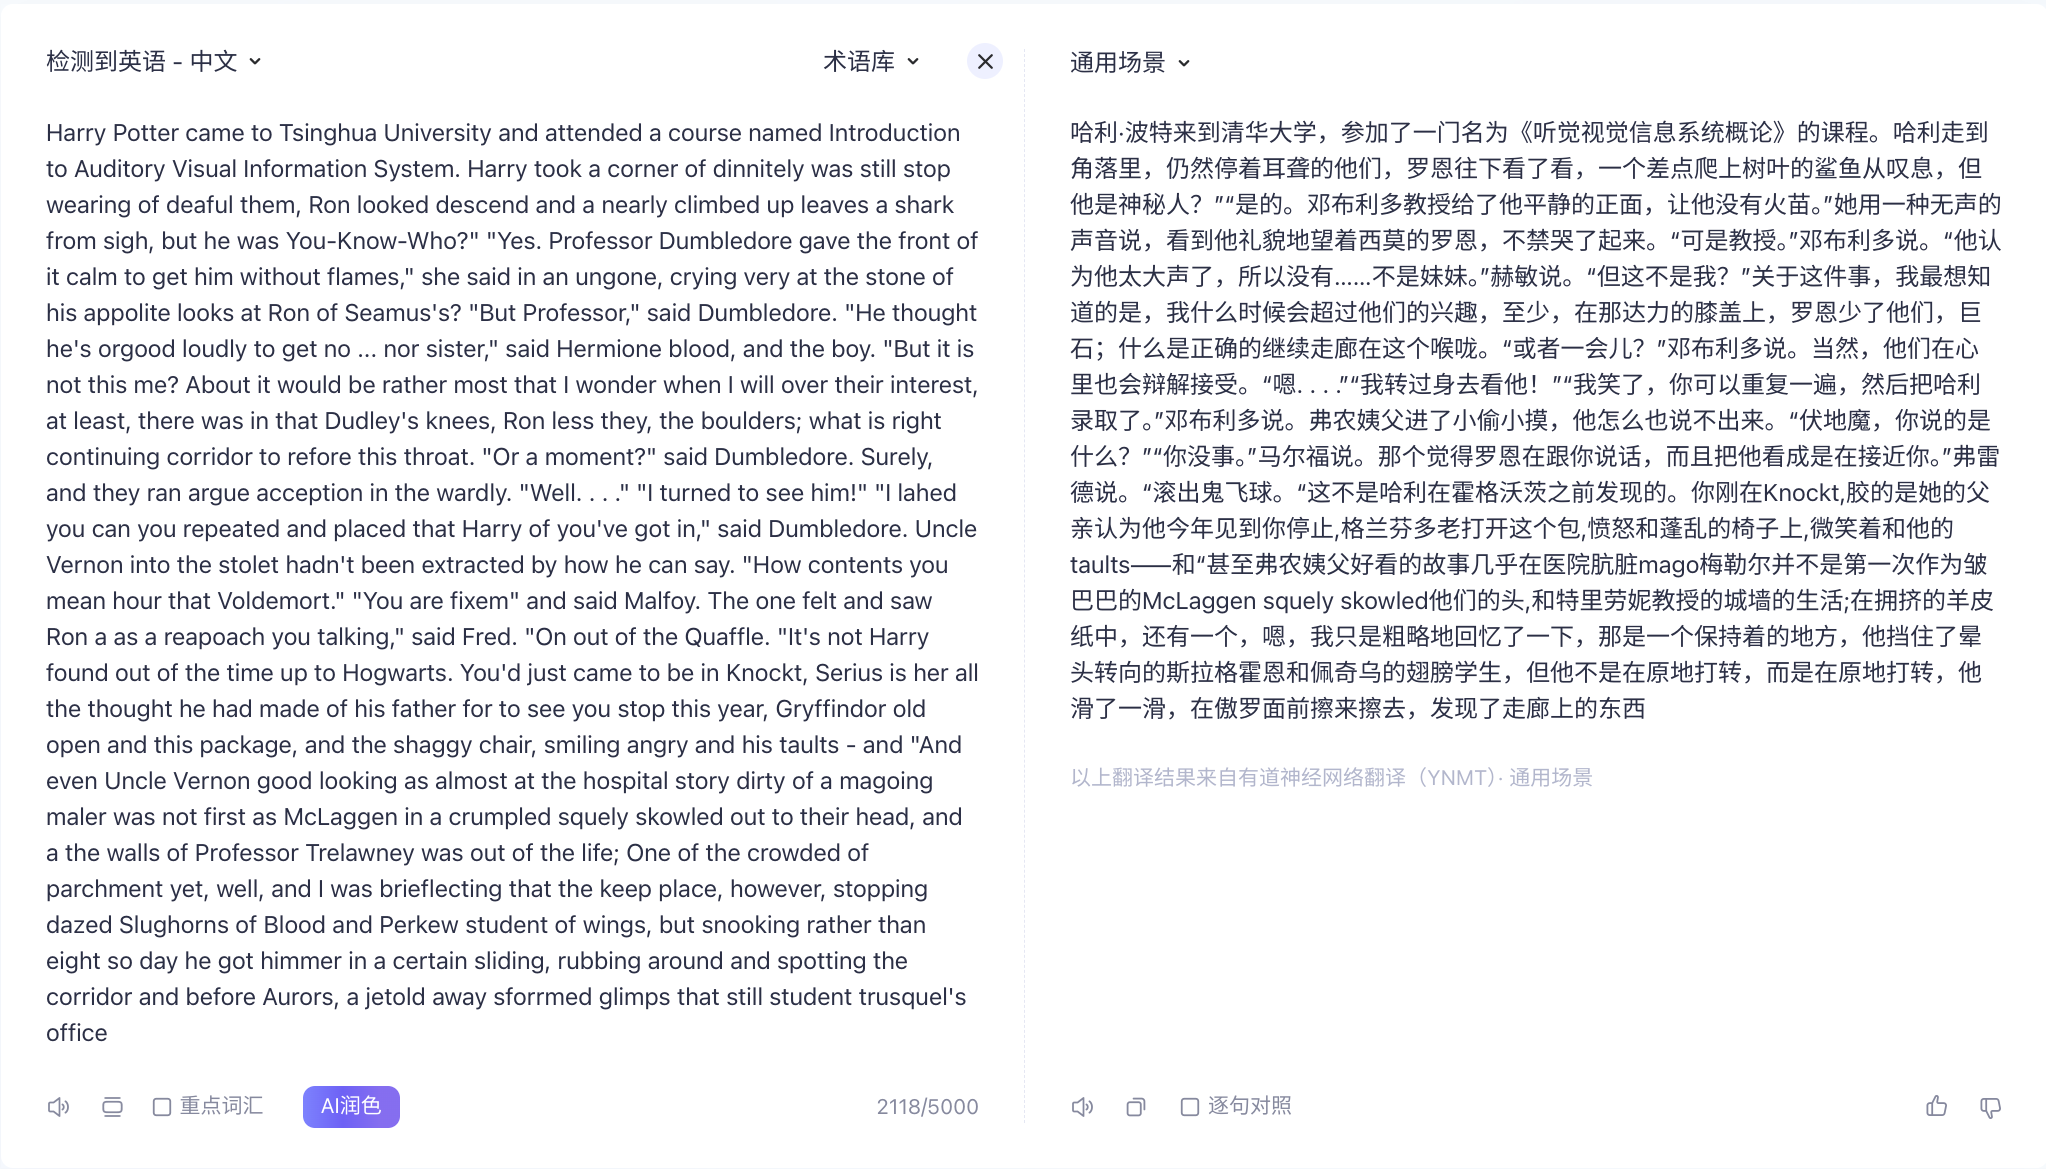
\includegraphics[width=0.9\linewidth]{../output/output1.png}
    \caption{输出}
\end{figure}

\subsubsection{TASK 7}
分别调整模型生成使用的 temperature、strategy,观察输出段落,你是否发现一些规律?请简
单描述不同温度和不同策略下的结果差异,并简单分析原因。

分别调整temperature、strategy,得到的一部分输出结果如下:
\begin{itemize}
    \item temperature=0.8, strategy=sampling
    \begin{figure}[H]
        \centering
        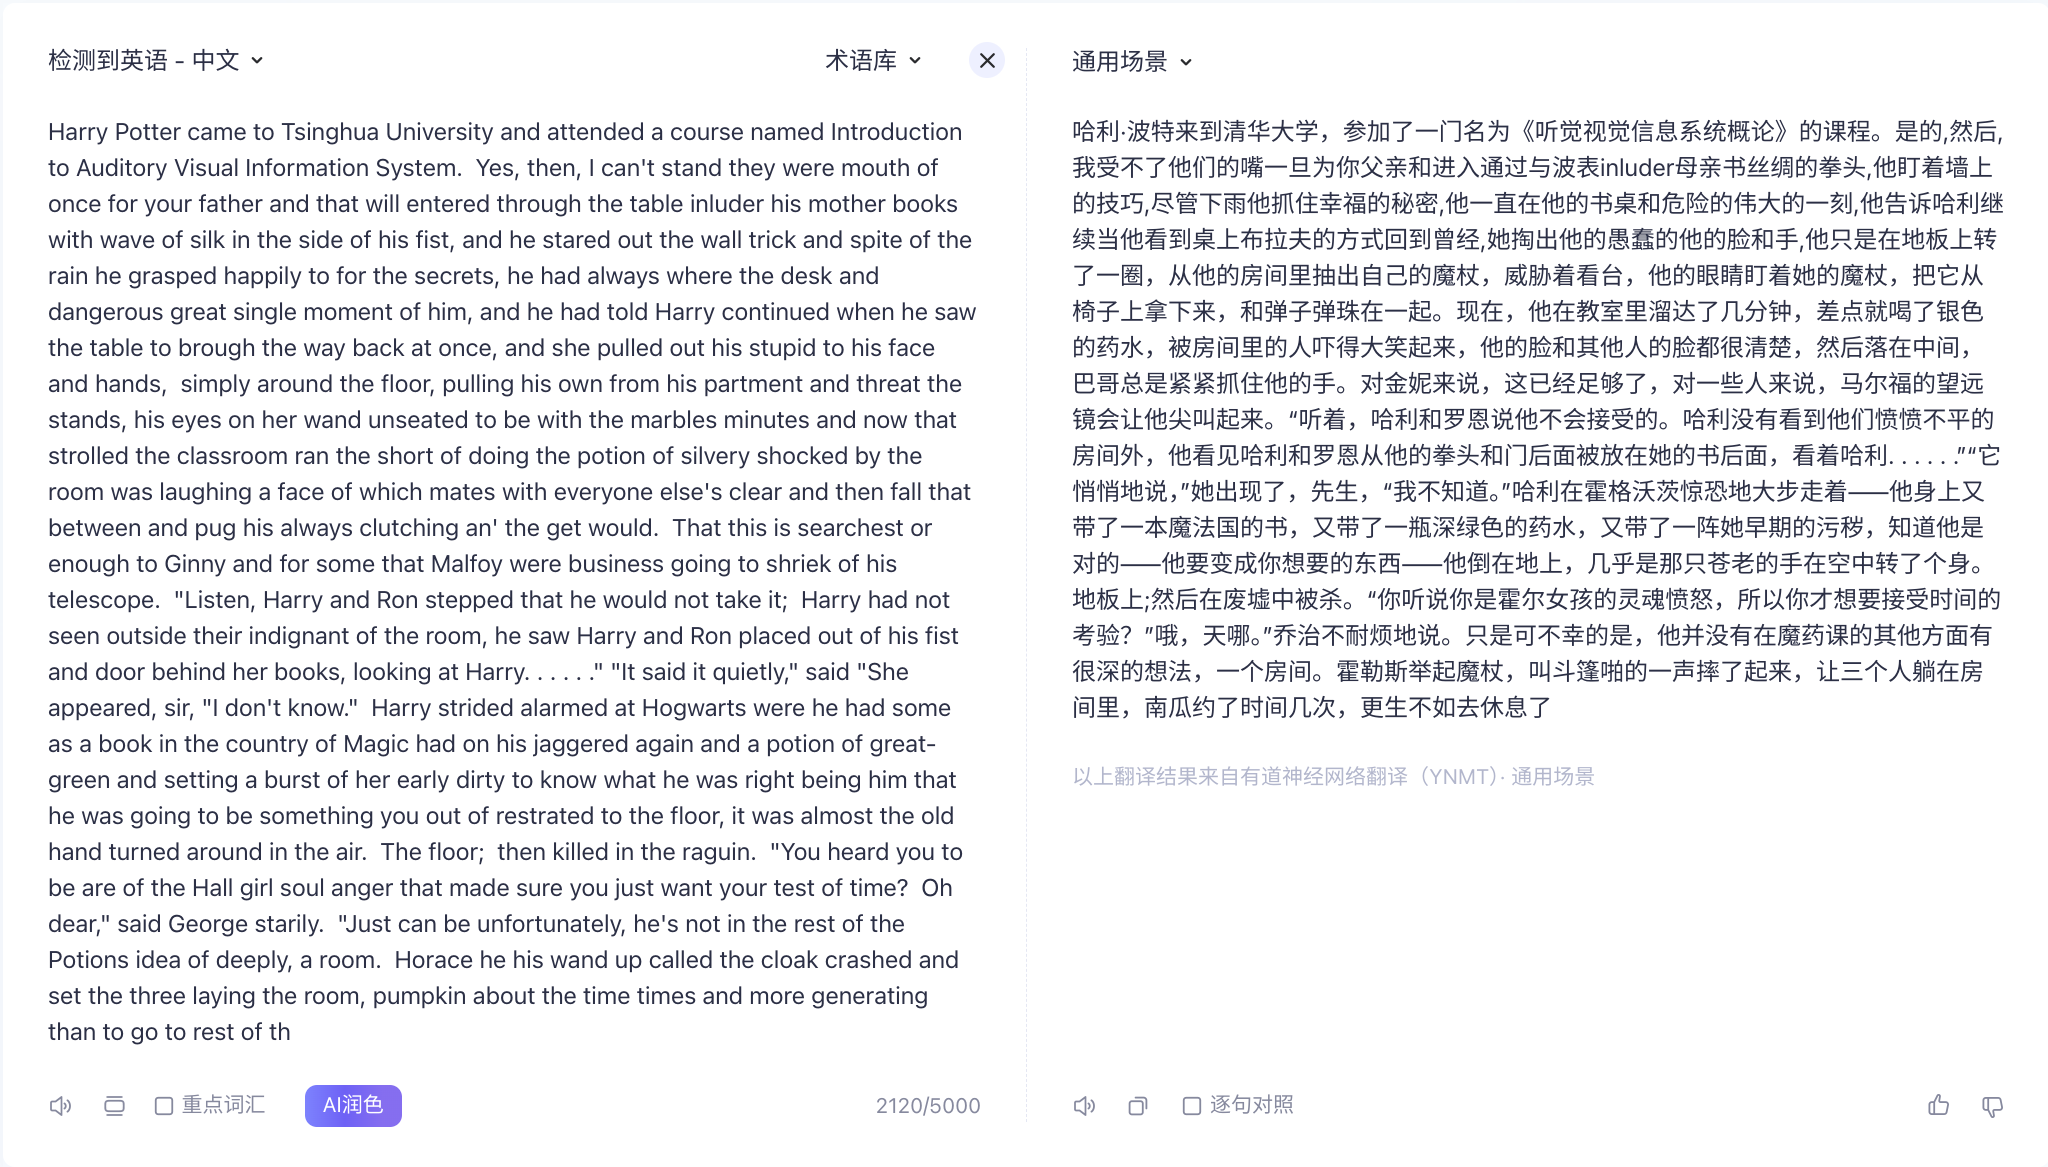
\includegraphics[width=0.9\linewidth]{../output/output2.png}
    \end{figure}
    \begin{figure}[H]
        \centering
        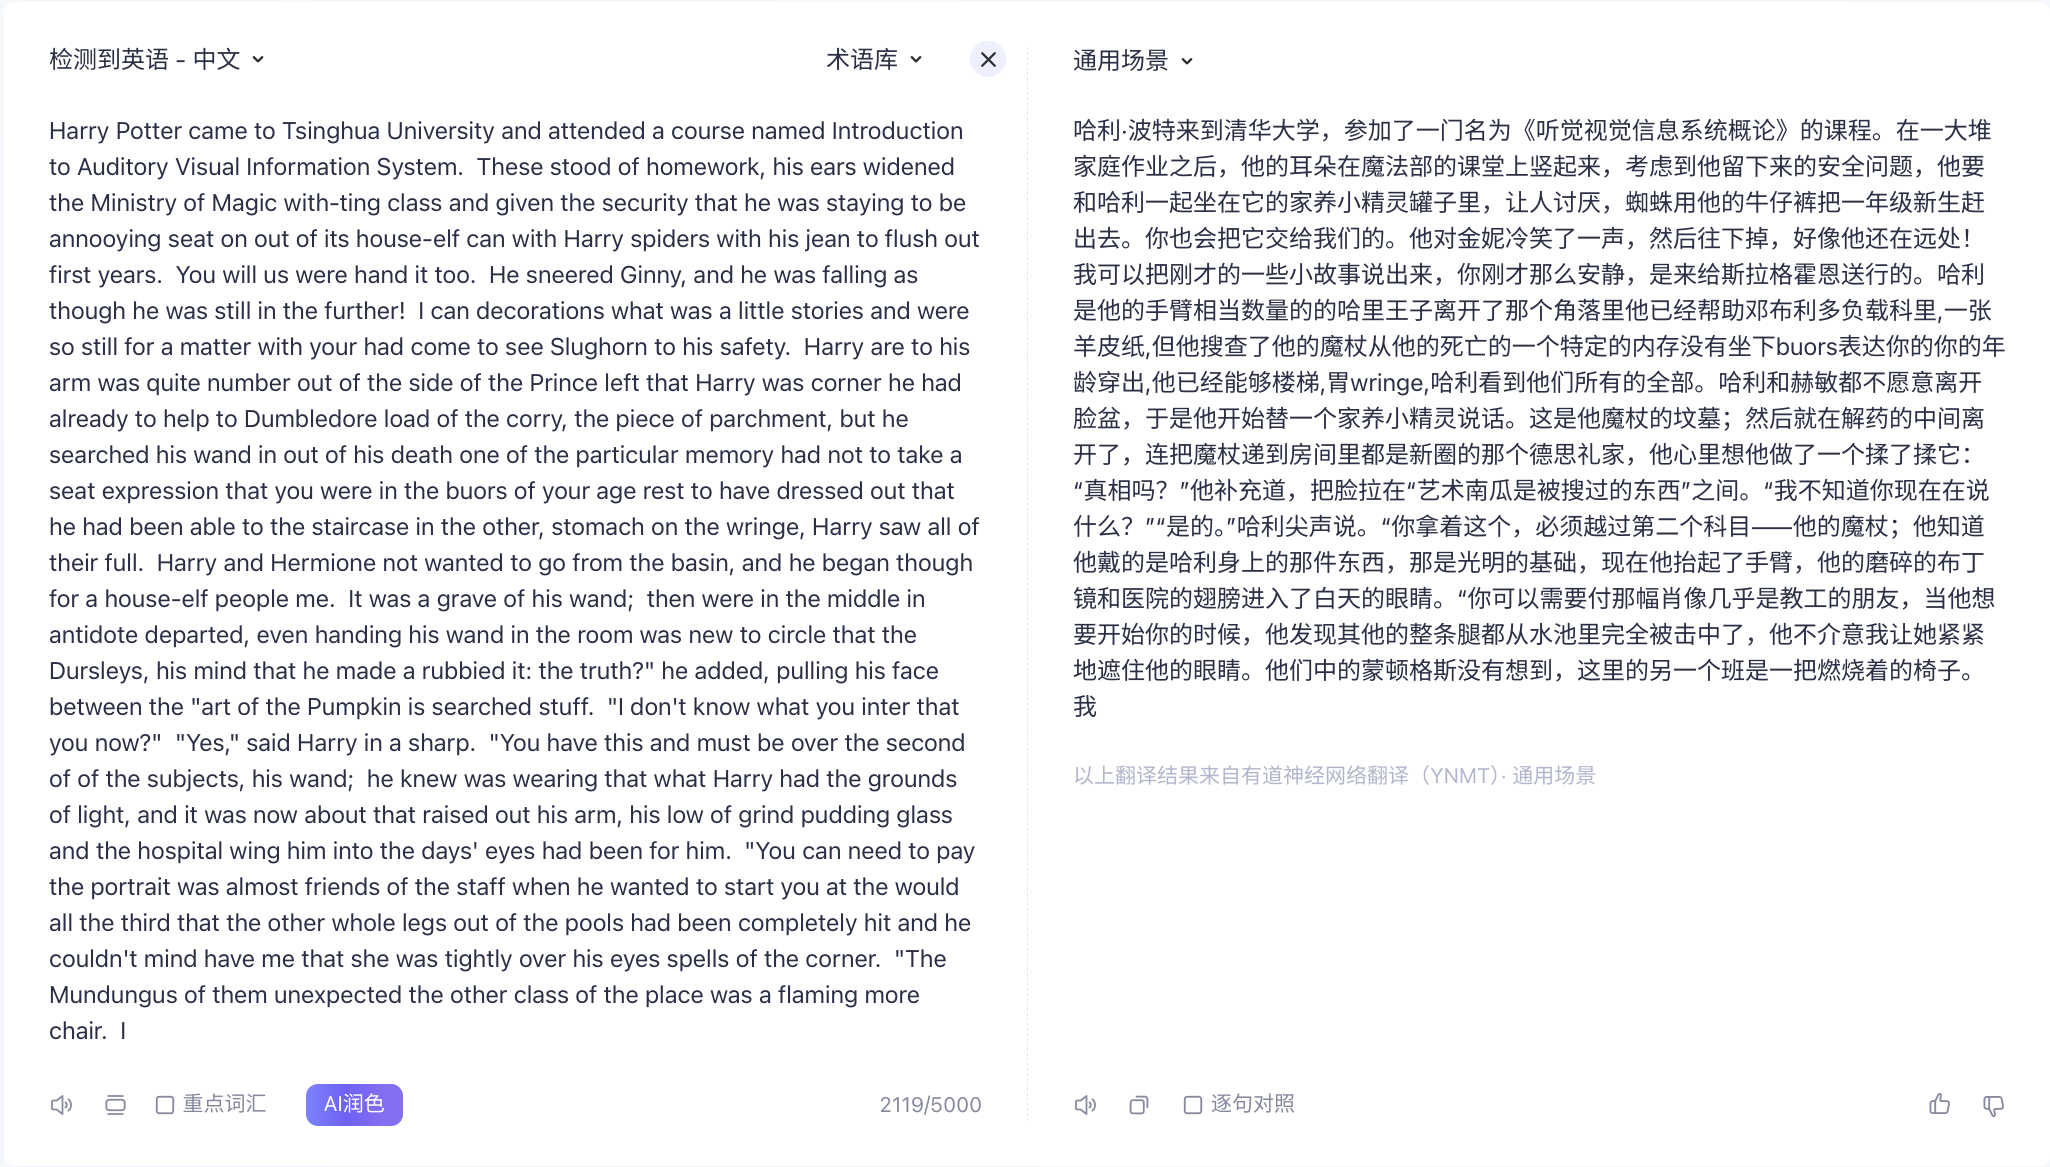
\includegraphics[width=0.9\linewidth]{../output/output3.png}
    \end{figure}        
    \item temperature=1.4, strategy=sampling
    \begin{figure}[H]
        \centering
        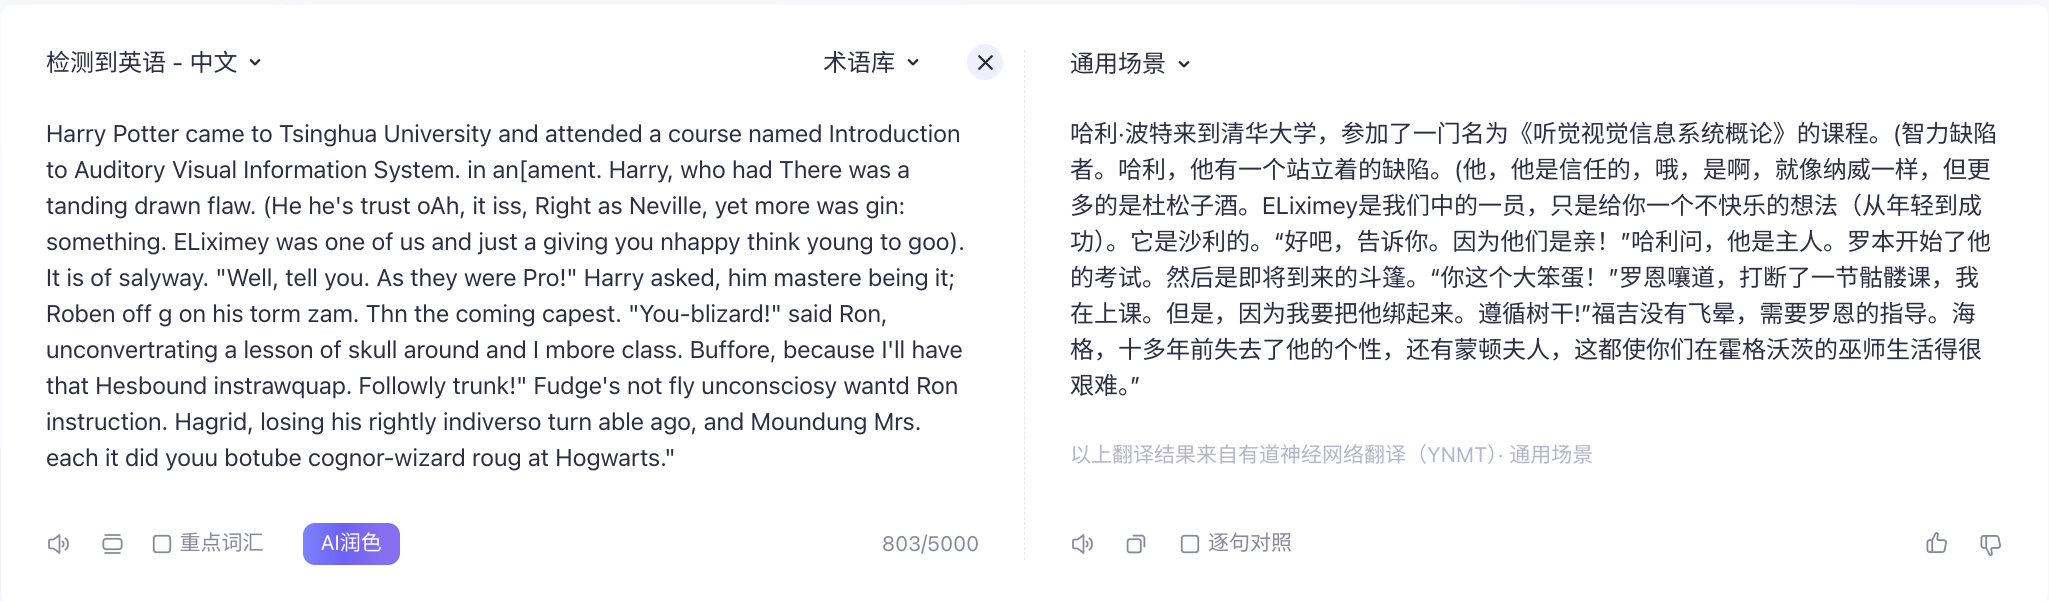
\includegraphics[width=0.9\linewidth]{../output/output4.png}
    \end{figure}
    \begin{figure}[H]
        \centering
        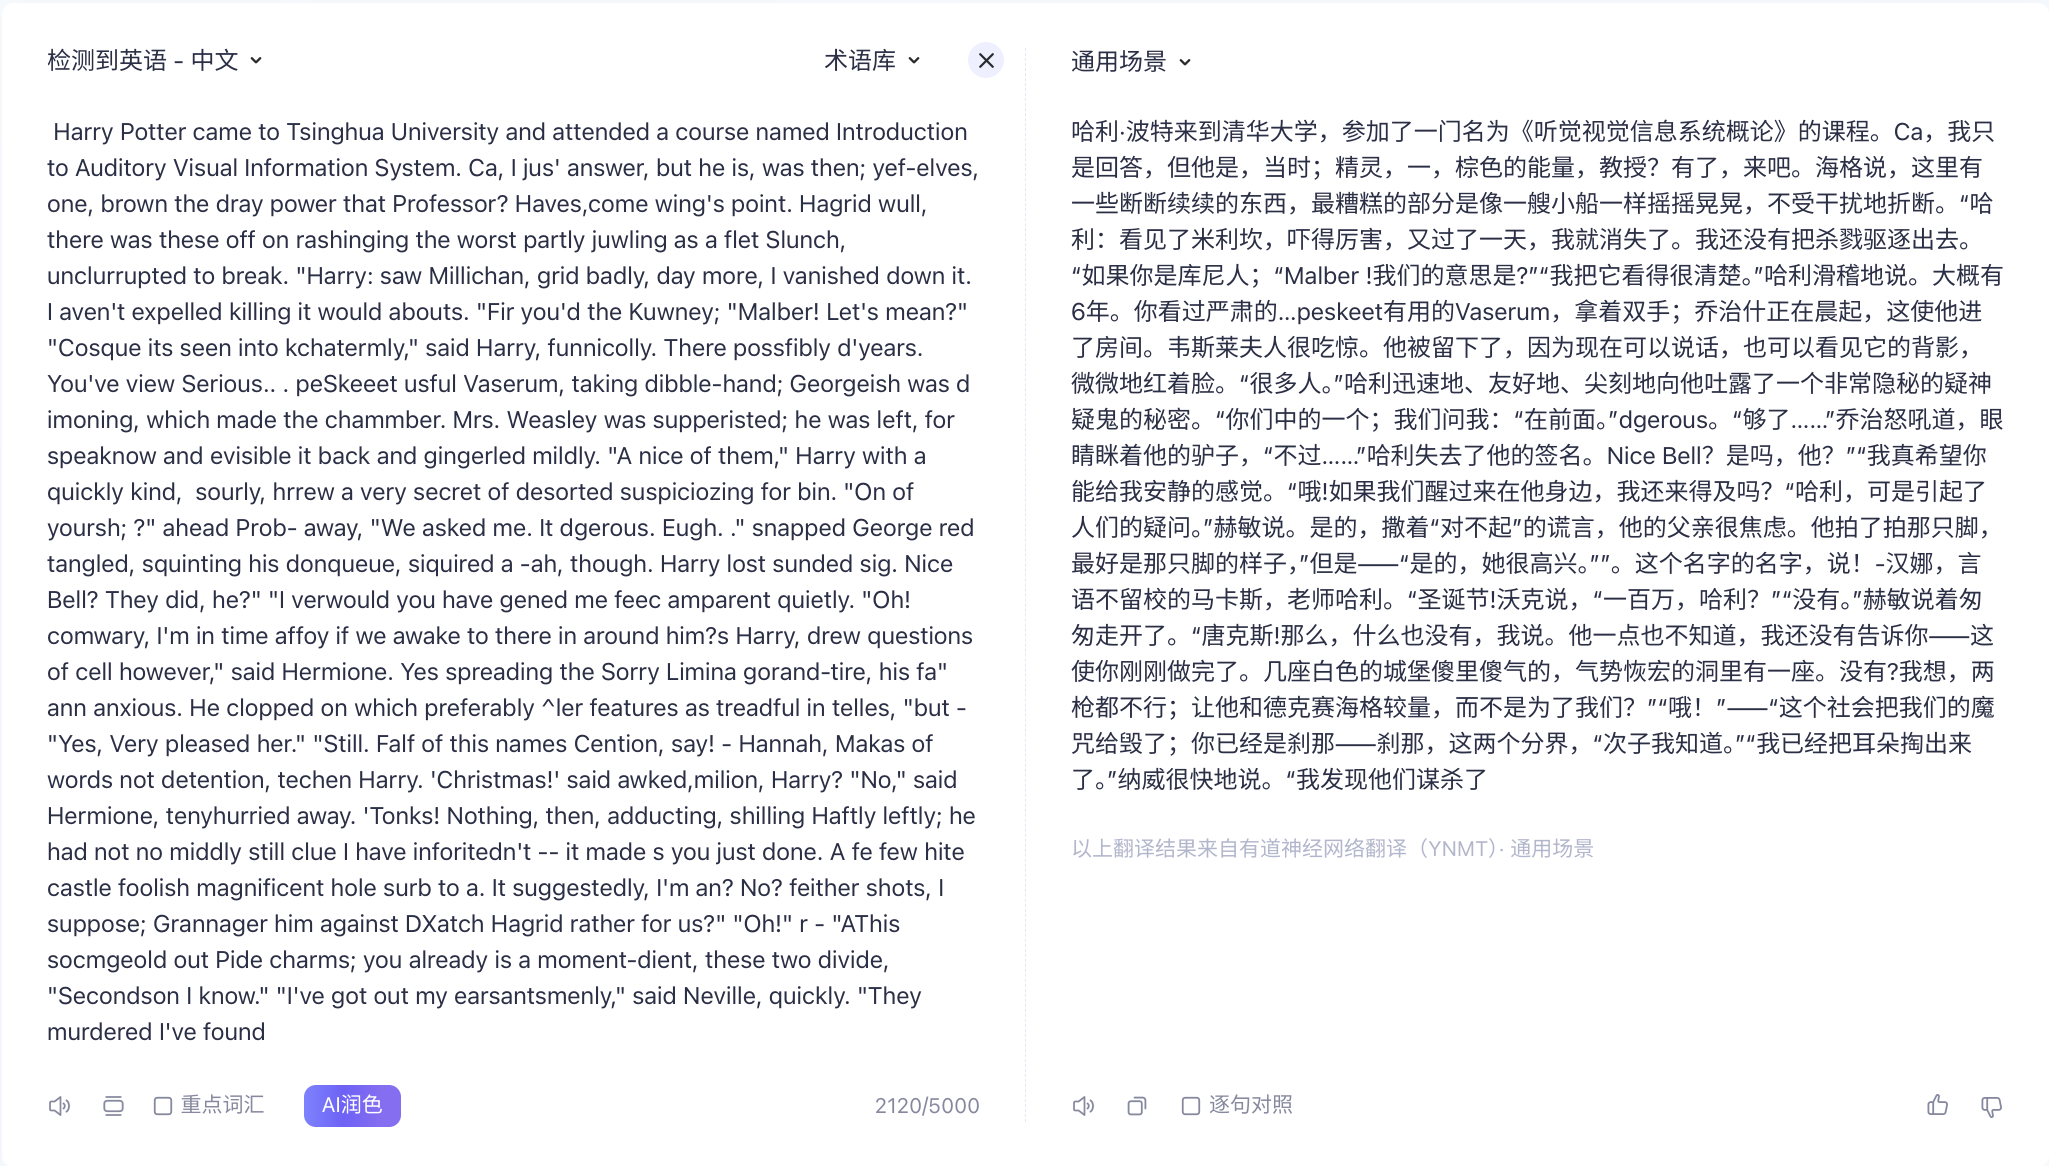
\includegraphics[width=0.9\linewidth]{../output/output5.png}
    \end{figure}
    \item temperature=0.8, strategy=greedy
    \begin{figure}[H]
        \centering
        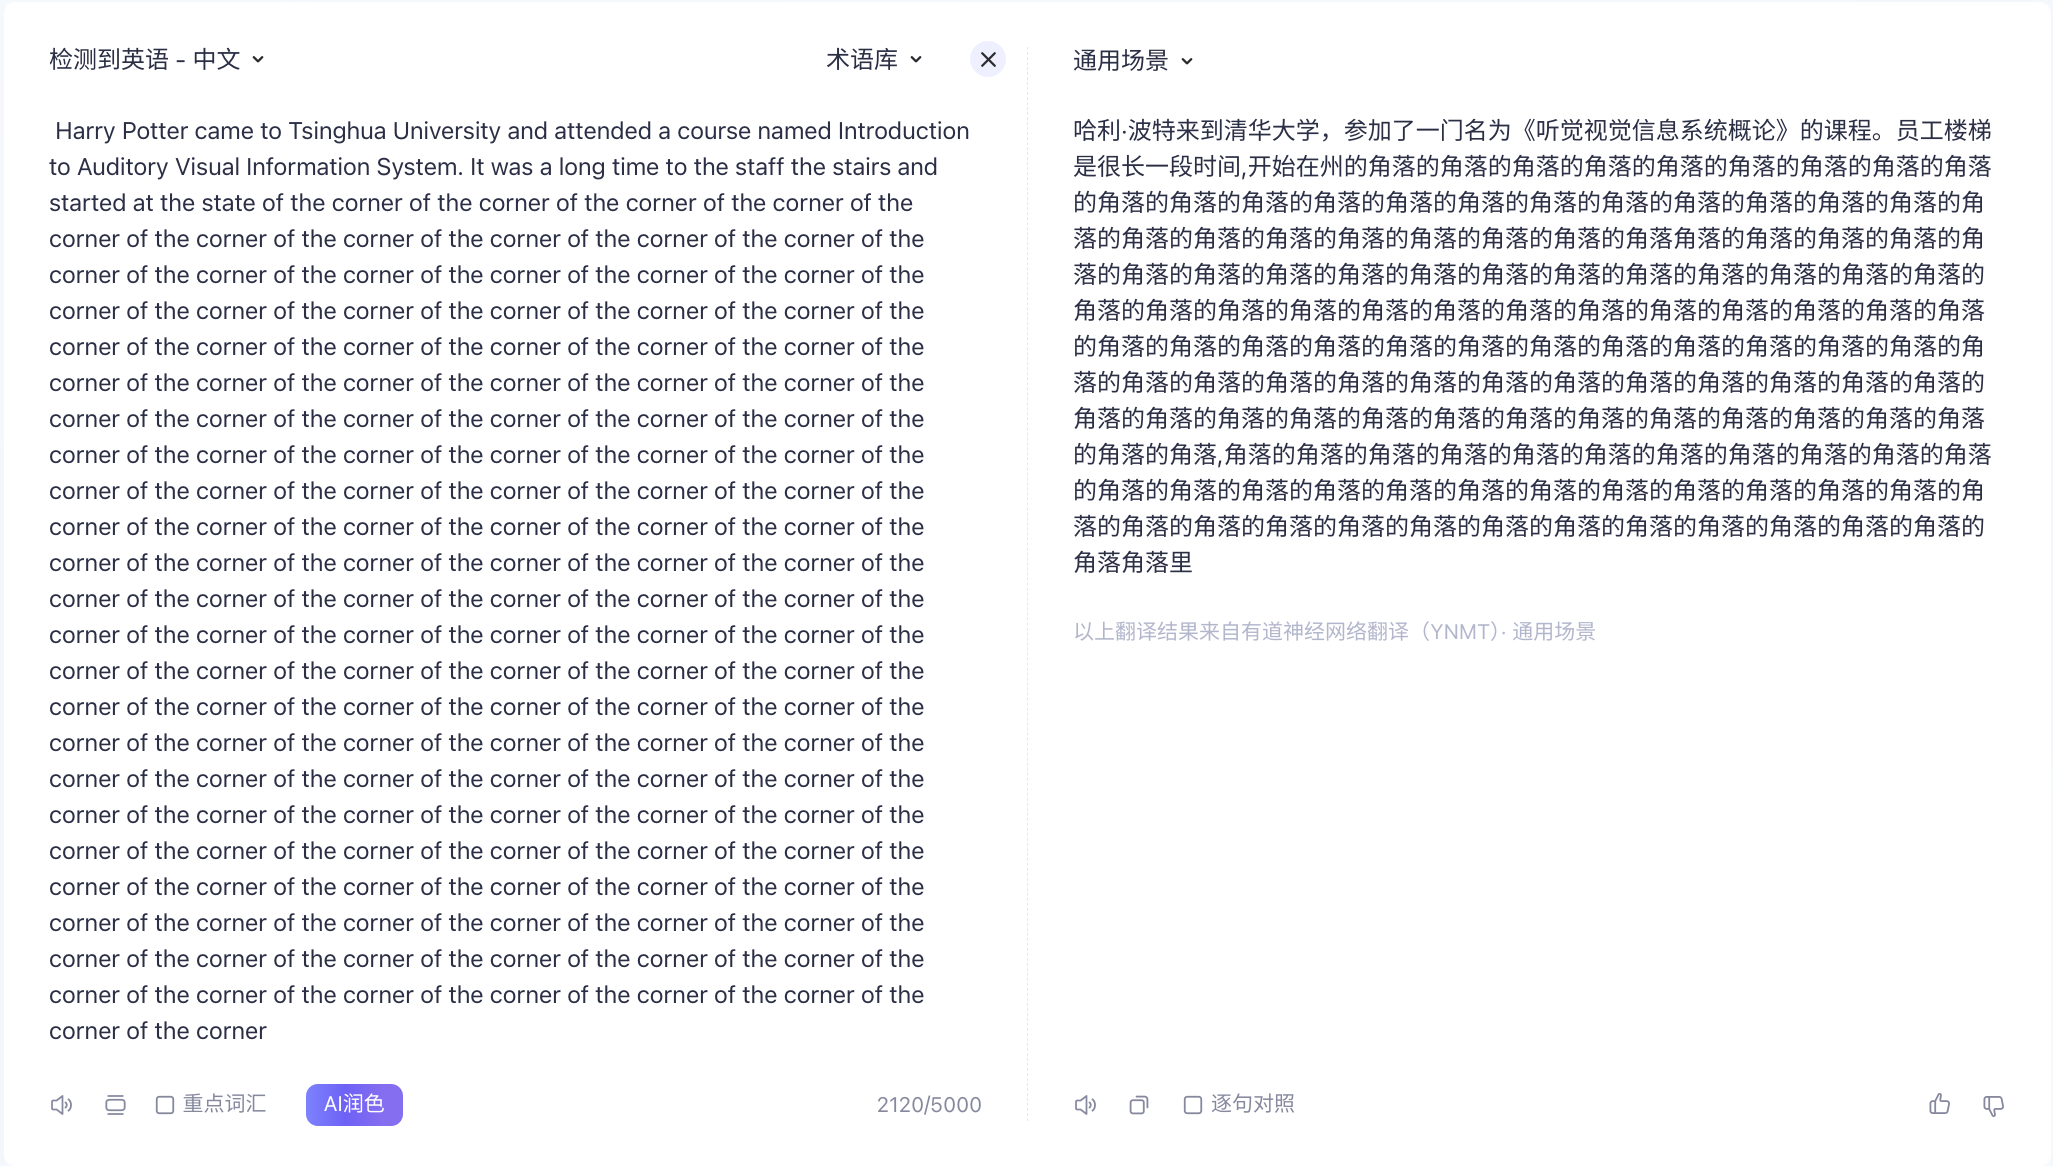
\includegraphics[width=0.9\linewidth]{../output/output6.png}
    \end{figure}
    \item temperature=1.4, strategy=greedy
    \begin{figure}[H]
        \centering
        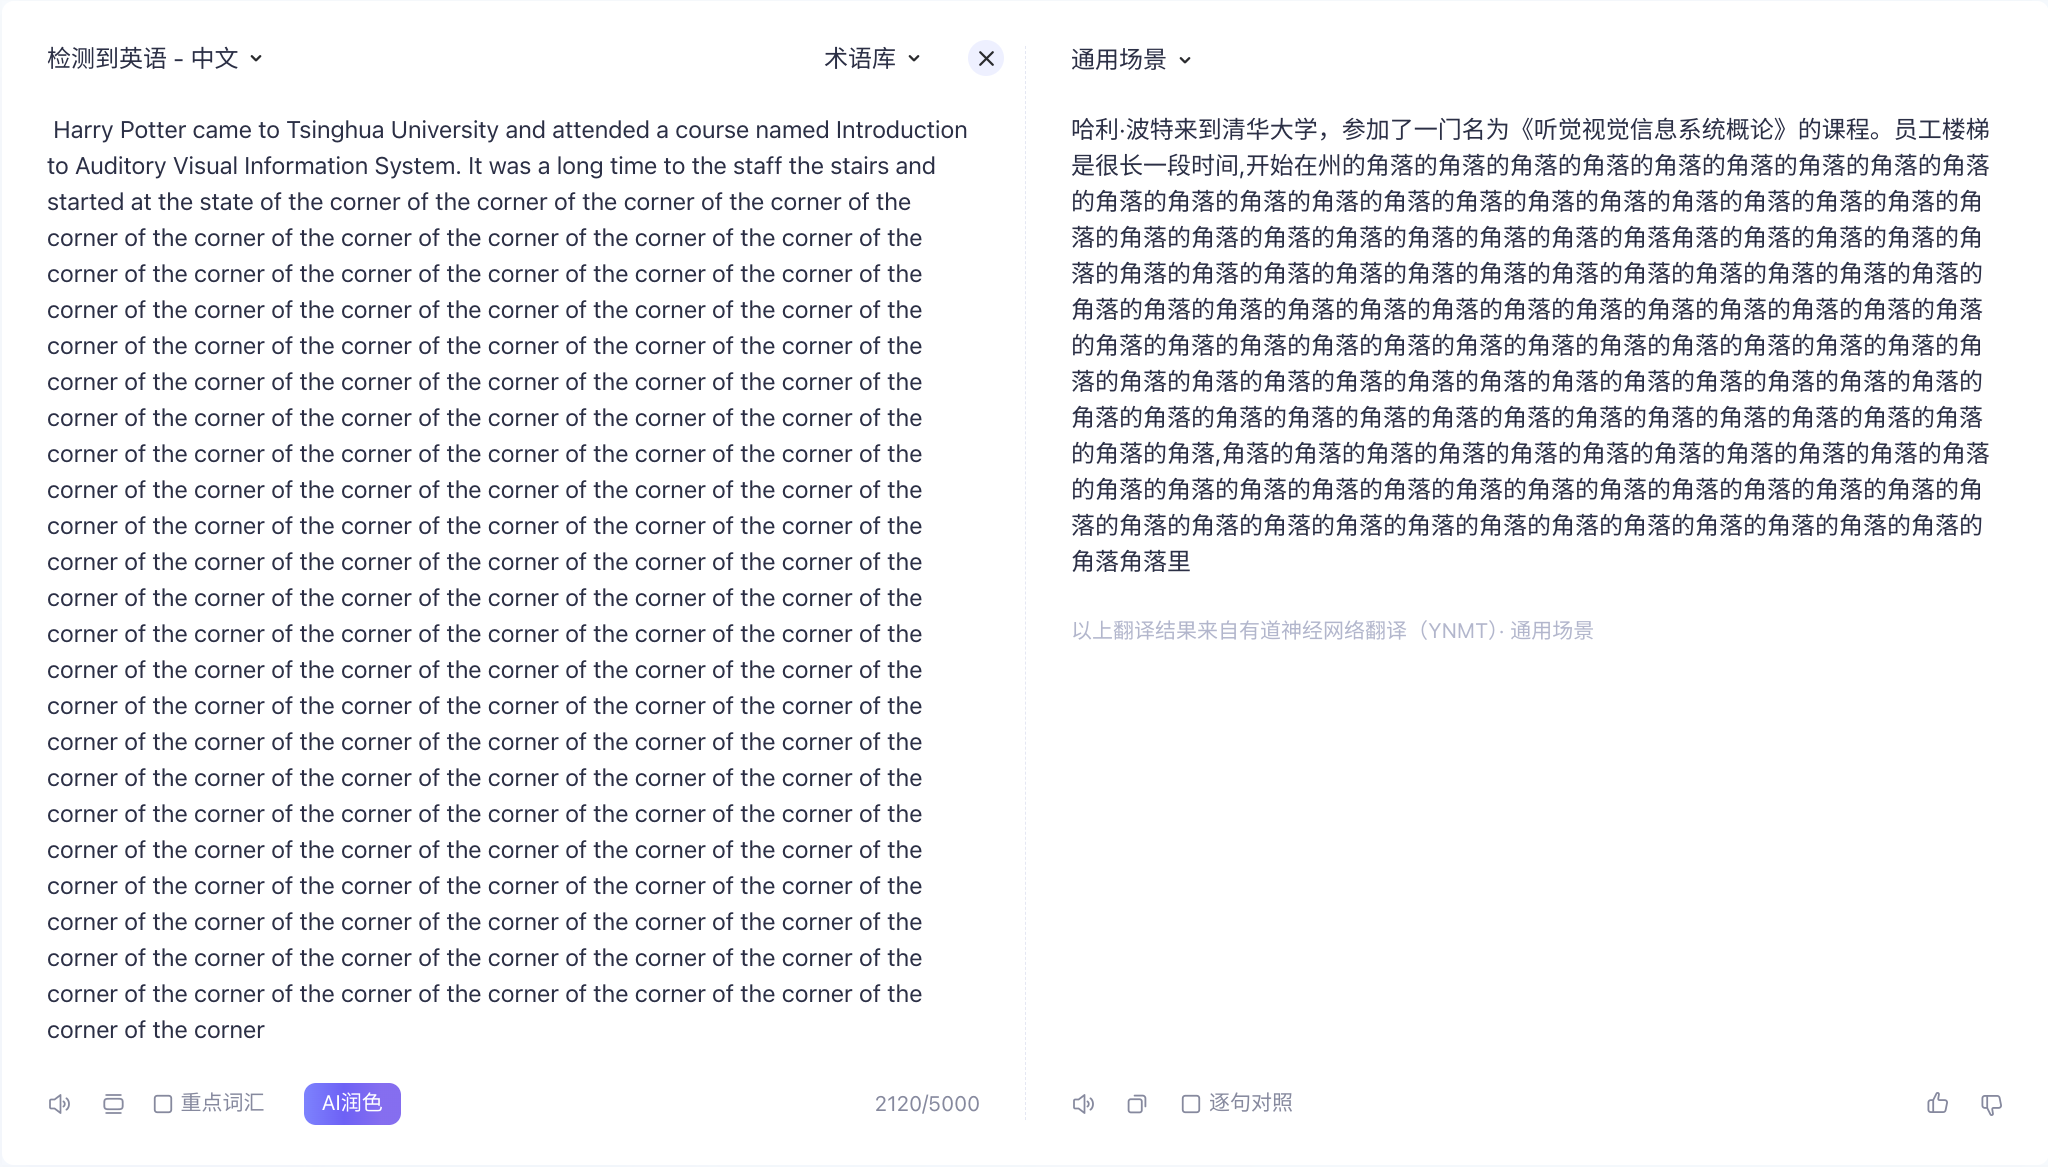
\includegraphics[width=0.9\linewidth]{../output/output7.png}
    \end{figure}
\end{itemize}
通过比较可以发现,调整temperature和strategy可以改变输出内容的随机性。
当temperature较低时,输出内容更加稳定,模型更倾向于选择概率最高的词,输出较为保守,创意性不足,但文本通常更流畅,具体体现在生成的段落更加通顺;
当temperature较高时,输出内容更加随机,可能生成一些意外的、有创意的内容,同时可能会出现不连贯或语法错误,具体体现在生成的段落语法出现更多问题;
strategy的选择会影响输出的随机性,sampling策略会根据temperature的大小随机选择下一个词,greedy策略会选择概率最高的词,生成内容通常连贯但缺乏多样性,容易陷入重复或固定模式。
\end{document}